\section{Design og arkitektur}

Dette kapittelet beskriver det tekniske oppsettet av prototypen -- hvilke teknologier
som er valgt, hvordan infrastrukturen er organisert, og hvordan endringer rulles ut
automatisk. Selve søke- og navigasjonsløsningene som er bygget oppå denne arkitekturen
beskrives i kapitlene~6 og~7.

\subsection{Teknologistack}

\begin{figure}[H]
    \centering
    \includesvg[width=1.0\textwidth]{Images/Figures/helsedirAiTechStack}
    \caption{Oversikt over teknologistacken som er benyttet i prototypen.}
    \label{fig:tech-stack}
\end{figure}

Figur~\ref{fig:tech-stack} viser en oversikt over de ulike komponentene i systemet.
\hyperlink{ord:frontend}{Frontend} er bygget med React~\cite{reactjs-docs} og TypeScript
og bruker Vite som byggverktøy. Grensesnittet følger Digdirs designsystem og kommuniserer
med \hyperlink{ord:backend}{backend} via et RESTful-API (Representational State Transfer).

\hyperlink{ord:backend}{Backend} er implementert i Python med
FastAPI-\hyperlink{ord:rammeverk}{rammeverket}~\cite{fastapi-docs}, et moderne
asynkront rammeverk som automatisk genererer API-dokumentasjon. Backend håndterer
søkespørringer, innhenting av innhold og logging av brukeratferd. Den er koblet til en
MySQL~8-database der innhold, søkelogg og klikkstatistikk lagres.

\paragraph{Helsedirektoratets API (HAPI)} er et eksternt REST-grensesnitt som gir
tilgang til faglig innhold publisert av Helsedirektoratet~\cite{helsedir-api-docs}.
Innholdet er strukturert etter type -- blant annet faglige anbefalinger, retningslinjer
og temautdrag. I prototypen brukes HAPI på to måter:

\begin{itemize}
    \item Frontend henter utdypende detaljfelter (f.eks.\ begrunnelse og
        styrkegradering for anbefalinger) direkte fra HAPI for innhold som ikke
        er fullstendig lagret i den lokale databasen.
    \item Backend tilbyr et \hyperlink{ord:proxy}{proxy}-endepunkt mot HAPI slik at
        API-nøkkelen ikke eksponeres i nettleseren.
\end{itemize}

%%%%
\subsection{Infrastruktur}

Prototypen er distribuert på en virtuell maskin i NTNUs OpenStack-baserte
skytjeneste (SkyHigh). Løsningen er tilgjengelig over internett via domenet
\texttt{https://vm.idatg2901-v26-helsdir.iaas.iik.ntnu.no/}. Dette kapittelet
beskriver den underliggende infrastrukturen, inkludert nettverkstopologi,
konfigurasjon av den virtuelle maskinen, containerisering av backend og
database, samt bruken av Nginx som reverse proxy.

\subsubsection{Nettverk og tilgjengelighet}

Den virtuelle maskinen er plassert i et privat nettverk
(\texttt{192.168.0.0/24}) opprettet i OpenStack. Nettverket er koblet til
det eksterne nettverket \textit{ntnu-global} via en virtuell ruter. En
flytende IP-adresse (\texttt{129.241.150.141}) er tilordnet instansen og
mappet til dens interne IP-adresse. Dette gjør serveren tilgjengelig fra
internett uten behov for VPN.

Arkitekturen følger et klassisk skyoppsett der trafikk går fra internett
til en offentlig IP-adresse, videre gjennom en virtuell ruter og inn til
en instans i et privat subnett. Figuren tilhørende denne seksjonen viser
denne sammenhengen mellom internett, OpenStack-nettverk, ruter og instans.

\subsubsection{Virtuell maskin og lagring}

Løsningen kjøres på én virtuell maskin med Ubuntu Server 24.04 som
operativsystem. Instansen er konfigurert med 6 virtuelle CPU-kjerner og
8~GB RAM. I tillegg er det tilknyttet et separat SSD-basert blokkvolum
på 256~GB for vedvarende lagring av applikasjonsdata og modeller.

VM-en fungerer som applikasjonsserver og kjører både webserver,
backend-applikasjon og database (i containere). Det er ikke benyttet
flere instanser, lastbalansering eller høytilgjengelighetsmekanismer.
Oppsettet representerer dermed en én-nodes arkitektur tilpasset
utvikling og demonstrasjon.

Tilgang til maskinen skjer via SSH med nøkkelbasert autentisering.
Passordinnlogging er deaktivert, og kun forhåndsautoriserte offentlige
nøkler gir tilgang.

\subsubsection{Containerisering av backend og database}

Backend-applikasjonen og databasen kjøres i Docker-containere som
administreres med Docker Compose. Databasen benytter MySQL~8 og kjører
i en egen container med vedvarende lagring gjennom et navngitt Docker-volum.
Databasen initialiseres automatisk ved første oppstart gjennom et
SQL-oppsettskript.

Backend-applikasjonen bygges fra prosjektets Dockerfile basert på
\texttt{python:3.11-slim} og kjøres med Uvicorn. Applikasjonen eksponerer
et \texttt{/health}-endepunkt som benyttes både av Docker og av eksterne
overvåkingsmekanismer for å verifisere at tjenesten er operativ.
Containeren starter først når databasen er bekreftet tilgjengelig.

Frontend kjøres ikke i container. Den bygges lokalt og distribueres som
statiske filer til \texttt{/var/www/app} på VM-en. Dette reduserer
kompleksiteten i deploy-prosessen og gjør at Nginx kan servere frontend
direkte.

\subsubsection{Nginx som reverse proxy}

Nginx er installert direkte på VM-en og fungerer som inngangspunkt for
all ekstern trafikk. HTTPS termineres i Nginx ved bruk av TLS-sertifikater
utstedt av Let's Encrypt. All HTTP-trafikk omdirigeres automatisk til HTTPS.

Nginx serverer frontend som statiske filer fra
\texttt{/var/www/app}, mens forespørsler til stien \texttt{/api}
videresendes til backend-containeren på \texttt{127.0.0.1:8000}.
Kommunikasjonen mellom Nginx og backend foregår internt på VM-en via HTTP.

Denne arkitekturen gjør at frontend og backend fremstår som én samlet
tjeneste for klienten, samtidig som backend isoleres bak reverse proxyen.
Løsningen unngår dermed CORS-relaterte problemstillinger og sentraliserer
håndtering av TLS og sikkerhetsinnstillinger.

\subsubsection{Konfigurasjon i OpenStack}

For å gjøre løsningen tilgjengelig fra internett er det konfigurert et
privat nettverk, en virtuell ruter mot \textit{ntnu-global} og en
flytende IP-adresse i OpenStack. Instansen er tilknyttet en egen
security group som tillater innkommende trafikk på portene 22 (SSH),
80 (HTTP), 443 (HTTPS), 3306 (MySQL) og 8000 (backend).

Portene 3306 og 8000 er åpne for å muliggjøre ekstern administrasjon
og testing i utviklingsfasen. I en produksjonssetting burde disse vært
begrenset til interne nettverk eller fjernet helt for å redusere
angrepsflaten.

\subsubsection{GitHub-integrasjon og CI/CD}

VM-en er konfigurert med en self-hosted GitHub Actions runner som muliggjør
automatisk bygging og utrulling av backend ved push til repositoryet.
Runneren kjører direkte på VM-en og har tilgang til Docker-miljøet,
slik at oppdatering av containere kan automatiseres.

Dette gir en enkel CI/CD-prosess der kodeendringer kan deployeres uten
manuell SSH-innlogging. Detaljer om workflow-konfigurasjon og
deploy-strategi beskrives i et senere kapittel.
%%%%%
\subsection{Infrastruktur}

\subsubsection{Virtuell maskin}

\begin{figure}[H]
    \centering
    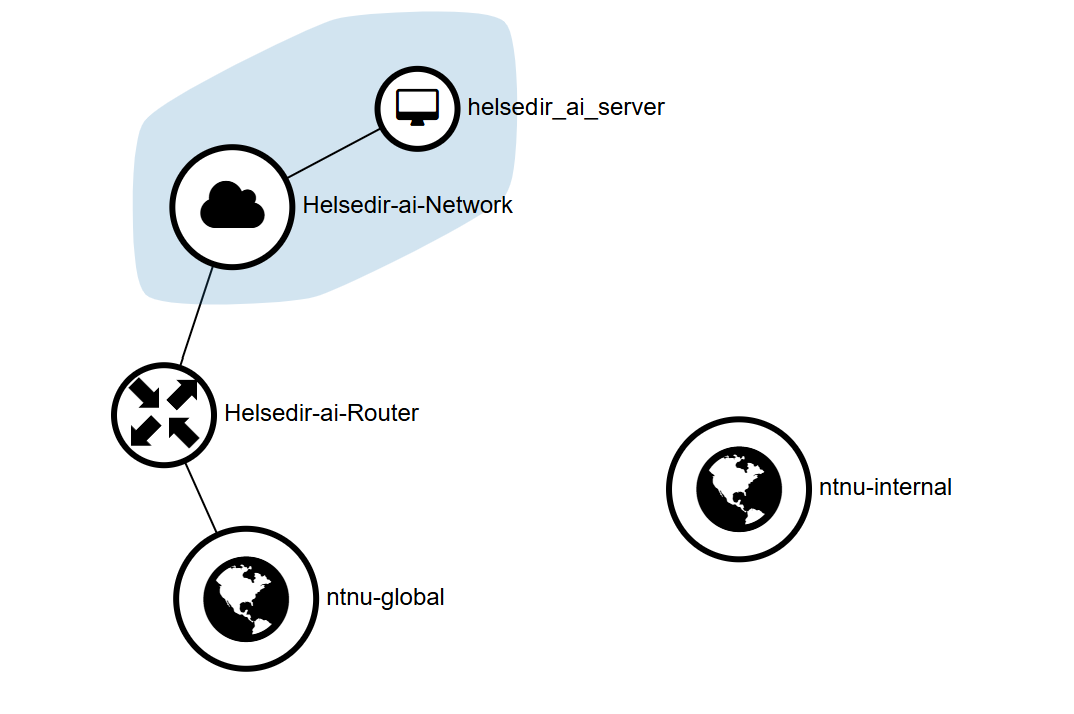
\includegraphics[width=\textwidth]{Images/helsedirektoratet.no/vm-netverk-graph.png}
    \caption{Topologien over hvordan VM-en er satt opp i SkyHigh på NTNUs globale nettverk.}
    \label{fig:vm-setup}
\end{figure}

Figur~\ref{fig:vm-setup} viser hvordan prototypen er kjørt på en virtuell maskin (VM)
med Ubuntu Linux i SkyHigh, NTNUs OpenStack-baserte skytjeneste. VM-en er koblet til
NTNUs globale nettverk slik at eksterne parter kan teste løsningene uten VPN.
Prototypen vil være tilgjengelig t.o.m. 21. juni.

\subsubsection{Containerisering med Docker}

Alle tjenester på VM-en kjøres som \hyperlink{ord:docker}{Docker}-containere~\cite{docker-docs}
og styres med \hyperlink{ord:docker-compose}{Docker~Compose}. Konfigurasjonen i
\texttt{docker-compose.yml} definerer to tjenester:

\begin{itemize}
    \item \textbf{db} -- MySQL~8-\hyperlink{ord:container}{container} med et vedvarende
        datavolum. Databasen initialiseres automatisk fra et SQL-oppsettskript ved første
        oppstart.
    \item \textbf{backend} -- Applikasjonscontainer bygget fra prosjektets
        \texttt{Dockerfile}. Kjører FastAPI via Uvicorn-serveren og starter
        ikke før \texttt{db}-containeren er bekreftet frisk (\textit{healthy}).
\end{itemize}

Begge containerne er konfigurert med helsesjekker. Backend eksponerer et
\texttt{/health}-endepunkt som Docker bruker til å bekrefte at tjenesten er
klar til å ta imot forespørsler.

\subsubsection{Nginx som reverse proxy}

På VM-en fungerer \hyperlink{ord:nginx}{Nginx}~\cite{nginx-docs} som
\hyperlink{ord:reverse-proxy}{reverse proxy} foran applikasjonen.
Frontend serveres statisk fra \texttt{/var/www/app}, mens alle forespørsler til stien
\texttt{/api} videresendes til backend-containeren på port~8000. Denne oppdelingen
gjør at frontend og backend fremstår som én tjeneste for nettleseren. HTTPS er aktivert
via NTNUs domene.

\subsection{CI/CD med GitHub Actions}

GitHub Actions~\cite{github-actions-docs} er brukt for å automatisere
kvalitetskontroll og utrulling (CI/CD -- Continuous Integration/Continuous Deployment).
Det er satt opp tre arbeidsflyter som til sammen utgjør en pipeline fra kodeendring til
kjørende produksjonstjeneste.

\paragraph{PR-byggsjekk} kjøres automatisk ved pull request mot
\texttt{dev}-grenen og kontrollerer at koden er fri for lint-feil og typeproblemer
før den merges, som vist i kode~\ref{kode:yaml-pr}:

\begin{lstlisting}[language=yaml,
    caption={GitHub Actions: PR-byggsjekk for frontend},
    label={kode:yaml-pr}]
name: PR Build Check
on:
  pull_request:
    branches: ["dev"]
jobs:
  prebuild-checks:
    runs-on: ubuntu-latest
    steps:
      - uses: actions/checkout@v4
      - uses: actions/setup-node@v4
        with:
          node-version: "20.19.0"
          cache: "npm"
      - run: npm ci
      - run: npm run lint
      - run: npx tsc --noEmit
\end{lstlisting}

\paragraph{Frontend-utrulling} kjøres automatisk når endringer merges til
\texttt{main}. Arbeidsflyten bygger applikasjonen, kopierer den til VM-en og
laster Nginx på nytt. Avslutningsvis kjøres en røyktest mot det offentlige
domenet for å bekrefte at tjenesten svarer, som vist i kode~\ref{kode:yaml-frontend}:

\begin{lstlisting}[language=yaml,
    caption={GitHub Actions: Utrulling av frontend},
    label={kode:yaml-frontend}]
name: Deploy frontend
on:
  push:
    branches: ["main"]
jobs:
  build-and-deploy:
    runs-on: [self-hosted, prod]
    steps:
      - uses: actions/checkout@v4
      - uses: actions/setup-node@v4
        with:
          node-version: "20"
          cache: "npm"
      - run: npm ci
      - name: Build
        env:
          VITE_API_BASE_URL: /api
          VITE_HELSEDIR_API_KEY: ${{ secrets.VITE_HELSEDIR_API_KEY }}
        run: npm run build
      - run: sudo rsync -a --delete dist/ /var/www/app/
      - run: sudo nginx -t && sudo systemctl reload nginx
      - run: curl -fsS https://vm.idatg2901-v26-helsdir.iaas.iik.ntnu.no/api/health
\end{lstlisting}

\paragraph{Backend-utrulling} henter nyeste kode fra Git og bygger
Docker-containeren på nytt. Arbeidsflyten venter deretter på at helsesjekken
godkjennes -- noe som sikrer at en mislykket oppdatering oppdages umiddelbart,
som vist i kode~\ref{kode:yaml-backend}:

\begin{lstlisting}[language=yaml,
    caption={GitHub Actions: Utrulling av backend},
    label={kode:yaml-backend}]
name: Deploy backend (prod)
on:
  push:
    branches: ["main"]
jobs:
  deploy:
    runs-on: [self-hosted, prod]
    steps:
      - name: Deploy on VM
        run: |
          cd /home/ubuntu/helsedir-ai-backend
          git fetch origin
          git reset --hard origin/main
          docker compose build backend
          docker compose up -d --no-deps backend
          for i in {1..100}; do
            status=$(docker inspect \
              -f '{{.State.Health.Status}}' helsedir-ai-backend)
            [ "$status" = "healthy" ] && exit 0
            [ "$status" = "unhealthy" ] && exit 1
            sleep 3
          done
\end{lstlisting}

Alle tre arbeidsflytene kjøres på en selvhostet GitHub Actions-runner
(\texttt{self-hosted, prod}) som er installert direkte på VM-en. Dette gjør at
utrulling skjer uten å sende kode over nettverket -- runneren har allerede tilgang
til det lokale filsystemet og Docker-miljøet på maskinen.

\subsubsection{Github runner hostet på VM}
